\chapter{Análisis}
En el presente capítulo se aborda un análisis exhaustivo de los principales problemas que afectan la calidad y sostenibilidad del software en proyectos de \Gls{mlopsg}, con un enfoque particular en \Gls{snapperml}. Para entender las dificultades y desafíos técnicos que enfrenta un sistema como \Gls{snapperml}, es fundamental examinar tanto el estado del arte de las herramientas de \Gls{mlopsg} y desarrollo web, como el concepto de \gls{deuda} y sus implicación en el desarrollo.

\section{Fundamentos y estado del arte}
En esta sección se presentan los fundamentos y el estado del arte relacionados con la gestión de experimentos de machine learning y el desarrollo web. Las herramientas de \Gls{mlopsg} han revolucionado la manera en que se gestionan, reproducen y optimizan los experimentos en proyectos de aprendizaje automático, mientras que las tecnologías modernas de frontend y backend continúan mejorando la experiencia de usuario y la eficiencia del desarrollo de aplicaciones web.

A lo largo de esta sección, se analizan las herramientas más utilizadas y sus principales características, destacando cómo se comparan y complementan entre sí. Esta revisión es esencial para establecer un contexto adecuado y justificar las decisiones tecnológicas tomadas en el desarrollo y optimización de \Gls{snapperml}.

\subsection{Herramientas para MLOps}
\begin{itemize}
    \item \textbf{MLflow} \cite{mlflow} : MLflow es una plataforma de código abierto que gestiona el ciclo de vida completo de un proyecto de machine learning, incluyendo la experimentación, la reproducibilidad, y el despliegue. MLflow consta de cuatro componentes principales:
          \begin{itemize}
              \item \textbf{Tracking}: Una API y una interfaz de usuario que permiten registrar experimentos, parámetros, métricas, artefactos, y otros metadatos de forma estructurada.
              \item \textbf{Projects}: Facilita el empaquetado y la distribución de proyectos ML en un formato estándar, como YAML, especificando las dependencias, el entorno, los parámetros y el punto de entrada del proyecto.
              \item \textbf{Models}: Permite empaquetar modelos de frameworks populares (TensorFlow, PyTorch, Scikit-Learn, etc.) en un formato unificado y almacenarlos en un registro de modelos. Además, proporciona soporte para el despliegue en múltiples entornos, como REST APIs.
              \item \textbf{Model Registry}: Un componente para gestionar el ciclo de vida de los modelos, incluyendo etapas de desarrollo, pruebas, y producción, con funciones de registro y control de versiones.
          \end{itemize}
    \item \textbf{Weights \& Biases} \cite{weightsandbiases}: Weights \& Biases (W\&B) es una herramienta popular para la experimentación y el seguimiento de modelos de machine learning. Ofrece funcionalidades avanzadas como la gestión de experimentos, la \gls{hpog}, y la visualización de métricas. W\&B se integra fácilmente con frameworks de ML y ofrece soporte para la colaboración en equipo, lo que permite a los usuarios compartir resultados y análisis.

    \item \textbf{Comet} \cite{cometml}: Comet proporciona una plataforma basada en la nube (con opciones de despliegue on-premise) para el seguimiento y la gestión de experimentos. Permite registrar y rastrear parámetros, métricas, artefactos, y resultados de manera estructurada. Entre sus características se incluyen soporte para cuadernos Jupyter, \gls{hpog}, y un sistema robusto de visualización. También permite monitorear métricas del sistema, como el uso de CPU y memoria, y se integra con múltiples lenguajes y frameworks.

    \item \textbf{Polyaxon} \cite{polyaxon}: Polyaxon es una plataforma de \Gls{mlopsg} enfocada en la gestión completa del ciclo de vida de los proyectos de ML. Utiliza Kubernetes para asegurar que los experimentos sean reproducibles, escalables y portables. Polyaxon permite definir y ejecutar experimentos complejos, optimizar hiperparámetros, gestionar métricas y parámetros, y desplegar modelos a producción. Además, cuenta con un sistema avanzado de manejo de usuarios y roles, lo que lo hace adecuado para grandes organizaciones.

    \item \textbf{Kubeflow} \cite{kubeflow}: Kubeflow es una plataforma de \Gls{mlopsg} que se enfoca principalmente en el despliegue de flujos de trabajo de ML en Kubernetes. Su objetivo es hacer que los proyectos de ML sean portables y escalables. Incluye Kubeflow Pipelines, que facilita la creación y ejecución de flujos de trabajo complejos de ML, y herramientas para gestionar modelos y datos. Kubeflow es altamente integrable con otras soluciones de \Gls{mlopsg}, haciendo que sea una opción poderosa para equipos que ya utilizan Kubernetes.

    \item \textbf{Amazon SageMaker} \cite{sagemaker}: Amazon SageMaker es la plataforma de ML de AWS que ofrece un conjunto de herramientas para cubrir todo el ciclo de vida del desarrollo de modelos. Incluye capacidades como gestión de datos, cuadernos Jupyter en la nube, registro y seguimiento de experimentos, \gls{hpog}, y despliegue de modelos con monitorización. Amazon SageMaker Studio proporciona un entorno de desarrollo integral para gestionar todos los aspectos de un proyecto de ML, y herramientas como SageMaker Debugger y SageMaker Autopilot automatizan y mejoran el desarrollo y la optimización de modelos.

    \item \textbf{Google Vertex AI} \cite{vertexai}: Vertex AI es la suite de herramientas de Google Cloud Platform para ML, que integra servicios como AutoML, la gestión de modelos, y el despliegue escalable. Vertex AI ofrece una interfaz unificada para gestionar experimentos, optimizar modelos, y realizar entrenamientos a gran escala. La plataforma se integra estrechamente con otros servicios de GCP, como BigQuery y Dataflow, para facilitar el manejo de datos a gran escala y el entrenamiento distribuido.

    \item \textbf{Azure Machine Learning} \cite{azure}: Azure ML es la plataforma de \Gls{mlopsg} de Microsoft que ofrece soporte para todas las etapas del ciclo de vida del ML, desde el entrenamiento y la experimentación hasta el despliegue y la monitorización. Incluye funcionalidades avanzadas como pipelines reproducibles, integración con servicios de datos de Azure, y soporte para el formato ONNX para la inferencia en múltiples entornos. Azure ML también ofrece soporte para la \gls{hpog} y un completo entorno de desarrollo colaborativo.

    \item \textbf{Neptune.ai} \cite{neptune}: Neptune.ai es una herramienta ligera pero poderosa para la gestión de experimentos de ML. Ofrece una interfaz intuitiva y una API en Python para registrar y rastrear experimentos, facilitando la comparación y el análisis de resultados. Neptune es compatible con diversos frameworks y permite una colaboración eficaz mediante la gestión de proyectos y el control de acceso basado en roles.

    \item \textbf{Data Version Control (DVC)} \cite{dvc}: DVC es una herramienta de gestión de versiones para datos y modelos en proyectos de ML. Permite rastrear y reproducir experimentos de manera similar a Git, pero optimizada para grandes volúmenes de datos. DVC es útil para proyectos que necesitan un control estricto sobre versiones de datos y modelos, facilitando la reproducibilidad y la colaboración en equipos de data science.
\end{itemize}
Las herramientas mencionadas ofrecen un conjunto diverso de funcionalidades que abordan las necesidades de los proyectos de \Gls{mlopsg}, desde la gestión y el seguimiento de experimentos hasta el control de versiones y el despliegue escalable de modelos.

% Please add the following required packages to your document preamble:
% \usepackage{graphicx}
% \usepackage[table,xcdraw]{xcolor}
% Beamer presentation requires \usepackage{colortbl} instead of \usepackage[table,xcdraw]{xcolor}
\begin{table}[]
    \centering
    \resizebox{\textwidth}{!}{%
        \begin{tabular}{|
                >{\columncolor[HTML]{EFEFEF}}l |c|c|c|c|c|c|c|}
            \hline
            \multicolumn{1}{|c|}{\cellcolor[HTML]{EFEFEF}\textbf{\begin{tabular}[c]{@{}c@{}}MLOPS\\ vs\\ Características\end{tabular}}} &
            \cellcolor[HTML]{EFEFEF}\textbf{\begin{tabular}[c]{@{}c@{}}Registro de \\ detalles de \\ hardware\end{tabular}}             &
            \cellcolor[HTML]{EFEFEF}\textbf{\begin{tabular}[c]{@{}c@{}}Control \\ estocástico \\ automático\end{tabular}}               &
            \cellcolor[HTML]{EFEFEF}\textbf{HPO}                                                                                        &
            \cellcolor[HTML]{EFEFEF}\textbf{\begin{tabular}[c]{@{}c@{}}Empaquetado \\ de proyectos\end{tabular}}                        &
            \cellcolor[HTML]{EFEFEF}\textbf{\begin{tabular}[c]{@{}c@{}}Ejecución \\ en \\ la nube o \\ en clusters\end{tabular}}        &
            \cellcolor[HTML]{EFEFEF}\textbf{\begin{tabular}[c]{@{}c@{}}Interfaz \\ web\end{tabular}}                                    &
            \cellcolor[HTML]{EFEFEF}\textbf{\begin{tabular}[c]{@{}c@{}}Código \\ abierto\end{tabular}}                                                                                         \\ \hline
            \cellcolor[HTML]{EFEFEF}\textbf{Snapper-ML}                                                                                 & Sí      & Sí & Sí & Sí      & Sí & Sí      & Sí      \\ \hline
            \cellcolor[HTML]{EFEFEF}\textbf{MLflow}                                                                                     & No      & a  & No & Sí      & Sí & Parcial & Sí      \\ \hline
            \textbf{Weights \& Biases}                                                                                                  & Sí      & No & Sí & No      & Sí & Sí      & No      \\ \hline
            \textbf{CometML}                                                                                                            & No      & No & Sí & Parcial & No & Sí      & No      \\ \hline
            \textbf{Polyaxon}                                                                                                           & No      & No & Sí & Sí      & Sí & Sí      & Híbrido \\ \hline
            \cellcolor[HTML]{EFEFEF}\textbf{Kubeflow}                                                                                   & No      & No & Sí & Sí      & Sí & Sí      & Sí      \\ \hline
            \textbf{\begin{tabular}[c]{@{}l@{}}Amazon \\ SageMaker\end{tabular}}                                                        & Parcial & No & Sí & Parcial & Sí & Sí      & No      \\ \hline
            \textbf{Google Vertex AI}                                                                                                   & Parcial & No & Sí & Sí      & Sí & Sí      & No      \\ \hline
            \textbf{\begin{tabular}[c]{@{}l@{}}Azure Machine \\ Learning\end{tabular}}                                                  & Parcial & No & Sí & Sí      & Sí & Sí      & No      \\ \hline
            {\color[HTML]{212529} \textbf{Neptune.ai}}                                                                                  & Sí      & No & Sí & No      & Sí & Sí      & Sí      \\ \hline
            {\color[HTML]{212529} \textbf{\begin{tabular}[c]{@{}l@{}}Data Version \\ Control (DVC)\end{tabular}}}                       & No      & No & No & Sí      & No & No      & Sí      \\ \hline
        \end{tabular}%
    }
    \caption{Comparación de herramientas MLOps destacadas}
    \label{mlops}
\end{table}

La tabla \ref{mlops} proporciona una comparación detallada de estas herramientas, resaltando características clave como el seguimiento de experimentos, la optimización de hiperparámetros y el soporte para la ejecución en entornos distribuidos. A continuación se describe las capacidades esenciales que estas herramientas pueden proporcionar, permitiendo a los equipos de data science seleccionar las opciones más adecuadas para sus flujos de trabajo específicos.
\begin{itemize}
    \item \textbf{Seguimiento de experimentos}: Capacidad para registrar y rastrear detalles de los experimentos, como parámetros, métricas y resultados.
    \item \textbf{Registro de detalles de hardware}: Funcionalidad para registrar información del hardware, como el uso de CPU y memoria, durante la ejecución de los experimentos.
    \item \textbf{Control automático de estocasticidad}: Herramienta para gestionar y registrar semillas aleatorias automáticamente, lo que garantiza la reproducibilidad de los experimentos.
    \item \textbf{Registro de dependencias}: Capacidad para registrar y gestionar las dependencias de software y bibliotecas necesarias para ejecutar los experimentos.
    \item \textbf{\acrfull{hpo}}: Soporte nativo para la \gls{hpog} mediante técnicas avanzadas, como la optimización bayesiana.
    \item \textbf{Empaquetado de proyectos}: Capacidad para empaquetar proyectos de ML en un formato reproducible, especificando el entorno, las dependencias y los puntos de entrada.
    \item \textbf{Ejecución en la nube o en clusters}: Soporte para ejecutar experimentos en la nube o en infraestructuras de clusters, ofreciendo escalabilidad y flexibilidad.
    \item \textbf{Interfaz web}: Presencia de una interfaz web que facilita la gestión y visualización de experimentos y resultados.
    \item \textbf{Código abierto}: Indica si la herramienta es de código abierto y puede ser modificada y utilizada libremente por la comunidad.
\end{itemize}

\subsection{Herramientas web}
\subsubsection{Frontend}
El desarrollo frontend continúa evolucionando con un enfoque en mejorar la experiencia del usuario, la eficiencia del desarrollo y la modularidad del código. En la encuesta de Stack Overflow de 2024, se destacan tecnologías clave que siguen definiendo el entorno del desarrollo frontend, con un énfasis creciente en frameworks modernos, herramientas de construcción optimizadas y estrategias avanzadas para la gestión de estado y la integración con backend.
\begin{itemize}
    \item \textbf{Frameworks y bibliotecas}: React.js lidera el panorama como una de las bibliotecas más populares para construir interfaces de usuario interactivas y componentes reutilizables, ideal para aplicaciones de una sola página (SPAs). Angular también sigue siendo una opción sólida, proporcionando una solución completa para aplicaciones web empresariales con su arquitectura basada en componentes y TypeScript. Vue.js continúa ganando adeptos gracias a su simplicidad y flexibilidad, permitiendo a los desarrolladores integrar progresivamente funcionalidades en sus proyectos.
    \item \textbf{Herramientas y optimización}: Tecnologías como Webpack y Vite mejoran la experiencia de desarrollo mediante la optimización del empaquetado de módulos y la recarga en caliente. Además, los desarrolladores recurren a Sass y Tailwind CSS para un control mejorado sobre los estilos y una gestión más eficiente de las hojas de estilo.
          \begin{figure*}[ht]
              \centering
              \begin{subfigure}[t]{0.45\textwidth}
                  \centering
                  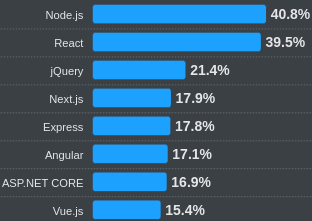
\includegraphics[width=\textwidth]{imagenes/survey_web_frameworks.png}
                  \caption{Sobre frameworks web.}
              \end{subfigure}%
              ~
              \begin{subfigure}[t]{0.5\textwidth}
                  \centering
                  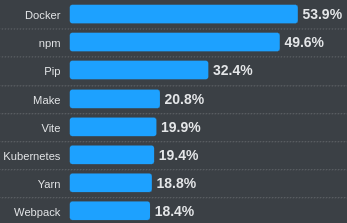
\includegraphics[width=\textwidth]{imagenes/survey_other_tools.png}
                  \caption{Sobre otras herramientas.}
              \end{subfigure}
              \caption{Resultados de la encuesta a desarrolladores de stackoverflow 2024 \cite{stackoverflow_survey}.}
          \end{figure*}

\end{itemize}

\subsubsection{Backend}
El desarrollo backend sigue siendo un componente crucial para las aplicaciones web modernas, proporcionando la lógica, la autenticación y las operaciones con bases de datos necesarias para aplicaciones robustas y escalables.
\begin{itemize}
    \item \textbf{Frameworks y entornos}: Express.js, un framework minimalista para Node.js, sigue siendo el favorito para crear aplicaciones de backend rápidas y escalables. También es frecuente el uso de NestJS, que se basa en TypeScript y aprovecha patrones de programación orientada a objetos y funcionales. Django y ASP.NET Core permanecen como opciones destacadas para aplicaciones más estructuradas, especialmente en proyectos que requieren características de seguridad y escalabilidad.
    \item \textbf{Bases de datos y gestión}: Las bases de datos relacionales como PostgreSQL y MySQL se combinan cada vez más con bases de datos NoSQL como MongoDB, lo que permite a los desarrolladores elegir modelos de datos que optimicen el rendimiento y la flexibilidad. Además, las arquitecturas basadas en microservicios están facilitando el uso de diferentes tecnologías de almacenamiento según las necesidades de la aplicación.
    \item \textbf{Infraestructura y despliegue}: Herramientas como Docker y Kubernetes son ahora fundamentales para la \textit{contenedorización} y orquestación de aplicaciones web, haciendo que el backend sea más fácil de escalar y desplegar en múltiples entornos. Las plataformas sin servidor, como AWS Lambda, están permitiendo una escalabilidad automática sin gestionar servidores físicos.
\end{itemize}

\begin{figure}[ht]
    \centering
    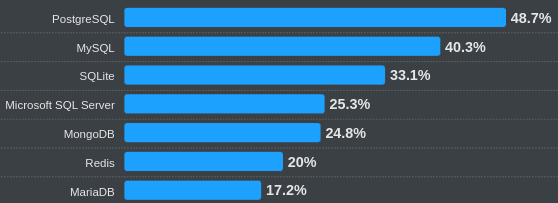
\includegraphics[width=0.8\textwidth]{imagenes/survey_database.png}
    \caption{Encuesta a desarrolladores de stackoverflow 2024 \cite{stackoverflow_survey} sobre bases de datos.}
\end{figure}

\section{Análisis de la Deuda Técnica}
La \Gls{deuda} es un concepto central en el desarrollo de software moderno, y entender sus causas, efectos y métodos de resolución resulta fundamental para la gestión eficaz de cualquier proyecto de software. En este capítulo se explora en profundidad el concepto de \gls{deuda}, su origen, indicadores, y métodos tanto de resolución como de prevención.

\subsection{¿Qué es la Deuda Técnica?}
El concepto de \gls{deuda} fue introducido en la década de 1990 por Ward Cunningham, uno de los autores del Manifiesto Ágil, para describir los compromisos técnicos que se adquieren cuando un equipo prioriza la entrega rápida de una funcionalidad o producto sobre una implementación ideal. En lugar de abordar las tareas necesarias para un código limpio y sostenible, como la refactorización y la optimización, los equipos pueden optar por soluciones rápidas que simplifiquen la entrega a corto plazo. Este tipo de decisiones, aunque a menudo inevitables, acumulan una \say{deuda} en el sistema que deberá \say{pagarse} en algún momento mediante el esfuerzo de corregir o mejorar el código.

Cunningham explicó la \gls{deuda} utilizando una analogía financiera, argumentando que las soluciones rápidas son como un préstamo que el equipo toma contra la calidad del código. Al igual que los intereses de un préstamo, las consecuencias de estos atajos se acumulan con el tiempo, haciendo que el código sea más difícil de mantener y aumentar su complejidad. Su célebre frase ilustra bien esta idea: \say{\textit{Si no hacemos que nuestro programa se alinee con lo que entendemos que es la manera adecuada de pensar sobre nuestros objetos financieros, seguiremos tropezando con esa inconsistencia, lo que es como pagar intereses en un préstamo}}\cite{introtodebt}.

Desde entonces, el término se ha popularizado y ampliado en la industria, evolucionando para abarcar una amplia variedad de situaciones en las que la calidad del software se ve comprometida en favor de la velocidad. En un sistema de software, la \gls{deuda} puede manifestarse en diversas áreas: código duplicado, arquitectura deficiente, falta de pruebas, documentación insuficiente, entre otros. Todos estos son \say{costos} que el equipo deberá enfrentar eventualmente si desea mantener una base de código estable y escalable.

Otros expertos en el campo, como Martin Fowler y el Software Engineering Institute, han desarrollado modelos para clasificar la \gls{deuda} en diferentes tipos y niveles, lo cual ayuda a los equipos a identificar y gestionar esta deuda de manera efectiva. La \gls{deuda} se reconoce ahora como un fenómeno inevitable en la mayoría de los proyectos de software, y su adecuada gestión es fundamental para el mantenimiento de la calidad y la sostenibilidad del software a largo plazo.

\subsection{Causas de la Deuda Técnica}
Existen diversas razones por las cuales puede generarse \gls{deuda} en un proyecto, y muchas veces no se debe únicamente a decisiones erróneas. Las principales causas incluyen:
\begin{itemize}
    \item \textbf{Plazos de Entrega Ajustados}: La presión por entregar rápidamente una funcionalidad o producto puede llevar a los equipos a adoptar atajos y soluciones rápidas, dejando de lado prácticas recomendadas de diseño y desarrollo.
    \item \textbf{Falta de Conocimiento o Experiencia}: Los desarrolladores, especialmente aquellos menos experimentados, pueden no estar al tanto de las buenas prácticas, lo que conlleva a decisiones técnicas que generan deuda. Esto es común en proyectos que evolucionan sin revisiones de código o mentoría adecuada.
    \item \textbf{Cambios en los Requisitos} La evolución de los requisitos puede hacer que decisiones técnicas previas se vuelvan obsoletas o no adecuadas. Este tipo de deuda se genera cuando el sistema debe adaptarse a nuevas funcionalidades o cambios en la arquitectura sin una refactorización previa.
    \item \textbf{Falta de Refactorización} La ausencia de una práctica regular de refactorización puede llevar a que el sistema acumule \gls{deuda} a medida que el código se vuelve menos limpio y más difícil de modificar.
\end{itemize}

\subsection{Indicadores de Deuda Técnica en un Proyecto}
La \gls{deuda} puede manifestarse en un proyecto de diferentes maneras. A continuación, se listan algunos de los principales signos de \gls{deuda}:

\begin{itemize}
    \item \textbf{Código duplicado}: la presencia de fragmentos de código repetidos puede indicar una falta de estructura y planificación en la arquitectura.
    \item \textbf{Baja cobertura de pruebas}: un sistema sin pruebas suficientes suele ser más frágil, costoso de mantener y difícil de modificar sin introducir errores.
    \item \textbf{Alta \gls{ciclomatica}}: funciones o métodos que contienen múltiples bifurcaciones y niveles de anidación incrementan la dificultad de comprensión y modificación del código.
    \item \textbf{Falta de documentación}: sin una documentación clara y completa, el código se vuelve difícil de entender y mantener, especialmente para nuevos desarrolladores en el equipo.
    \item \textbf{Desacople inadecuado}: dependencias mal estructuradas entre componentes del sistema que dificultan su modificación y evolución.
\end{itemize}

\subsection{Clasificación de la Deuda Técnica}

Existen diferentes enfoques para clasificar la \gls{deuda} en los proyectos de software. Cada clasificación proporciona una perspectiva única sobre el tipo de deuda que puede acumularse y sobre cómo gestionarla. A continuación, se exploran dos enfoques reconocidos: los tipos de \Gls{deuda} identificados por el Software Engineering Institute y el Cuadrante de la \Gls{deuda} de Martin Fowler.

\subsubsection{Tipos de Deuda Técnica según el Software Engineering Institute}
Según el documento publicado por el Software Engineering Institute titulado \say{Towards an Ontology of Terms on Technical Debt \cite{debtontology}}, existen trece tipos distintos de \gls{deuda}, cada uno asociado con indicadores clave que permiten su identificación en un proyecto. A continuación, se presenta una descripción de cada tipo de \gls{deuda}, con ejemplos ilustrativos.
\begin{itemize}
    \item \textbf{Architecture Debt}: Se refiere a problemas o limitaciones en la estructura general del sistema. Ejemplo: un sistema que utiliza una arquitectura monolítica enfrenta dificultades para escalar o actualizarse, generando costos adicionales cuando es necesario realizar cambios significativos.

    \item \textbf{Build Debt}: Implica la falta de optimización en el proceso de compilación o construcción de software. Ejemplo: tiempos de compilación excesivos que ralentizan el flujo de trabajo de los desarrolladores y aumentan el tiempo necesario para pruebas y despliegue.

    \item \textbf{Code Debt}: Hace referencia a la mala calidad del código en términos de legibilidad y mantenimiento. Ejemplo: código altamente duplicado o con complejidad innecesaria que hace difícil la realización de cambios sin introducir errores.

    \item \textbf{Defect Debt}: Incluye errores conocidos en el sistema que aún no han sido corregidos. Ejemplo: defectos menores en el código que no afectan directamente la funcionalidad principal, pero que acumulados pueden hacer que el sistema sea más frágil y difícil de mantener.

    \item \textbf{Design Debt}: Se genera cuando las decisiones de diseño no se alinean con los objetivos de largo plazo del sistema. Ejemplo: una interfaz de usuario que no sigue patrones de diseño modernos puede afectar la experiencia de usuario y requerir rediseño en fases futuras.

    \item \textbf{Documentation Debt}: Surge cuando la documentación está incompleta, desactualizada o es inexistente. Ejemplo: módulos de código críticos sin documentación detallada, lo que dificulta que nuevos desarrolladores comprendan y mantengan el sistema.

    \item \textbf{Infrastructure Debt}: Se refiere a problemas en la infraestructura de hardware o software en la que se basa el sistema. Ejemplo: servidores obsoletos o configuraciones de red que limitan la escalabilidad del sistema y necesitan ser actualizados.

    \item \textbf{People Debt}: Relacionado con la falta de habilidades, conocimiento o experiencia en el equipo de desarrollo. Ejemplo: un equipo que carece de experiencia en buenas prácticas de seguridad de software, lo que aumenta el riesgo de vulnerabilidades en el sistema.

    \item \textbf{Process Debt}: Ocurre cuando los procesos de desarrollo son ineficientes o no están bien definidos. Ejemplo: un flujo de trabajo sin revisiones de código formalizadas, lo que facilita la introducción de errores y de prácticas de desarrollo deficientes.

    \item \textbf{Requirement Debt}: Surge cuando los requisitos iniciales no se definen claramente o cambian sin una adecuada gestión. Ejemplo: funcionalidades que se agregan sin una evaluación de impacto, lo que puede generar inconsistencias o problemas de compatibilidad.

    \item \textbf{Service Debt}: Involucra problemas en los servicios externos o en las dependencias del sistema. Ejemplo: una aplicación que depende de un servicio de terceros que no ofrece disponibilidad continua, afectando la confiabilidad del sistema.

    \item \textbf{Test Automation Debt}: Corresponde a la falta de automatización de pruebas en el sistema. Ejemplo: la ausencia de pruebas automatizadas, que dificulta el despliegue continuo y aumenta el tiempo necesario para verificar que el sistema funcione correctamente.

    \item \textbf{Test Debt}: Se refiere a la falta de cobertura de pruebas para validar el comportamiento del sistema. Ejemplo: módulos críticos sin pruebas unitarias o de integración, lo cual incrementa el riesgo de que cambios futuros generen errores no detectados.
\end{itemize}

\subsubsection{Cuadrante de la Deuda Técnica de Martin Fowler}

Martin Fowler propuso otra forma de clasificar la \gls{deuda} mediante el \say{Cuadrante de la \Gls{deuda}}, el cual se basa en dos dimensiones: la intención de la deuda (deliberada o inadvertida) y la forma en que esta se gestiona (imprudente o prudente).

\begin{figure}[H]
    \centering
    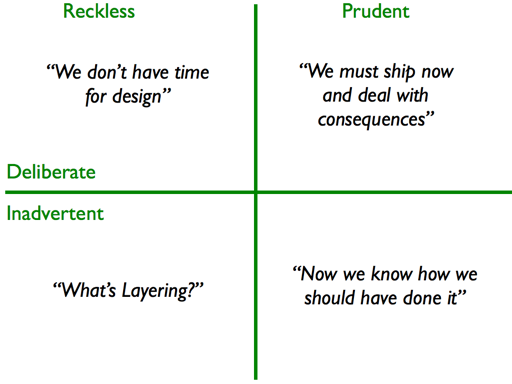
\includegraphics[width=0.7\textwidth]{imagenes/techDebtQuadrant.png}
    \caption{Technical Debt Quadrant by Martin Fowler.}
\end{figure}

Este modelo permite a los equipos de desarrollo comprender mejor la naturaleza de la \gls{deuda} y el enfoque adecuado para gestionarla. Las cuatro categorías de \gls{deuda} en este modelo son:
\begin{itemize}
    \item \textbf{Reckless-Deliberate (Imprudente y Deliberada)}: La \gls{deuda} se asume de manera consciente pero sin considerar las consecuencias a largo plazo. Ejemplo: omitir el diseño para ahorrar tiempo, diciendo: \say{No tenemos tiempo para el diseño}. Aunque permite avanzar rápidamente, esta decisión puede llevar a problemas de mantenimiento importantes.

    \item \textbf{Prudent-Deliberate (Prudente y Deliberada)}: La \gls{deuda} se asume de manera consciente y planificada, con la intención de abordarla en el futuro. Ejemplo: \say{Debemos lanzar ahora y lidiar con las consecuencias}, donde se prioriza el tiempo de entrega con la intención de refactorizar luego.

    \item \textbf{Reckless-Inadvertent (Imprudente e Inadvertida)}: La \gls{deuda} se incurre sin intención ni conocimiento, y de forma imprudente. Esto ocurre cuando el equipo carece de experiencia o conocimiento técnico. Ejemplo: un desarrollador que desconoce conceptos básicos de diseño, como la capa de abstracción, y toma decisiones que complican el sistema.

    \item \textbf{Prudent-Inadvertent (Prudente e Inadvertida)}: La \gls{deuda} ocurre sin que el equipo lo note inicialmente, pero es reconocida y abordada después. Ejemplo: \say{Ahora sabemos cómo deberíamos haberlo hecho}, donde el equipo identifica una mejor forma de resolver el problema después de implementar la solución inicial.
\end{itemize}

Este modelo ayuda a los equipos a tomar decisiones informadas sobre cómo gestionar la \gls{deuda}. Las deudas imprudentes, tanto deliberadas como inadvertidas, son generalmente críticas y deben priorizarse, mientras que las deudas prudentes pueden ser gestionadas con una planificación a largo plazo.

\subsubsection{Conclusión}

Ambos enfoques de clasificación de \gls{deuda} proporcionan a los equipos una perspectiva amplia para entender y gestionar los distintos tipos de deuda. Los trece tipos de \gls{deuda} permiten una identificación precisa de problemas específicos en el sistema, mientras que el Cuadrante de Fowler proporciona un marco para evaluar la intencionalidad y gestión de la deuda, facilitando la toma de decisiones sobre su resolución. Juntos, estos modelos permiten una gestión integral de la \gls{deuda}, ayudando a los equipos a mantener la calidad y sostenibilidad del software a lo largo del tiempo.

\subsection{Ejemplos de Deuda Técnica}

Para ilustrar la \gls{deuda} en el desarrollo de software, a continuación se presentan algunos ejemplos comunes, tanto en términos generales como en organizaciones que han enfrentado problemas significativos debido a la \gls{deuda}.

\subsubsection{Ejemplos Comunes de Deuda Técnica}

\begin{itemize}
    \item \textbf{Código legacy sin documentación}: A menudo, el código escrito hace muchos años carece de documentación y pruebas, lo que dificulta su modificación.
    \item \textbf{Sistemas monolíticos}: Proyectos antiguos suelen estar organizados de forma monolítica, lo que incrementa la complejidad al realizar cambios o al escalar funcionalidades.
    \item \textbf{Parches rápidos}: La aplicación de \say{parches} temporales para corregir errores críticos puede resolver problemas a corto plazo, pero si no se revisan, se convierten en problemas mayores.
\end{itemize}

\subsubsection{Ejemplos de empresas u organizaciones que han sufrido Deuda Técnica}

\begin{itemize}
    \item \textbf{X (Twitter)}: Ha enfrentado problemas de escalabilidad y rendimiento debido a la \gls{deuda} acumulada en sus sistemas iniciales.
    \item \textbf{NASA}: En algunos proyectos espaciales, la \gls{deuda} ha sido un problema debido a las limitaciones de hardware y a la evolución de los sistemas operativos y software con el tiempo. \item \textbf{Microsoft}: En varias versiones de Windows, Microsoft ha lidiado con la \gls{deuda} para garantizar la compatibilidad con software y hardware antiguos.
\end{itemize}

\subsection{Resolución de la Deuda Técnica}
La resolución de la \gls{deuda} requiere un esfuerzo consciente y constante. Algunas de las estrategias más efectivas para abordar la \gls{deuda} incluyen:

\begin{itemize}
    \item \textbf{Refactorización}: La refactorización es una técnica que permite mejorar el diseño y la estructura del código sin cambiar su funcionalidad. Mediante la refactorización, es posible reducir la complejidad, mejorar la legibilidad y eliminar duplicación de código.
    \item \textbf{Implementación de Pruebas Automatizadas}: Agregar pruebas automatizadas asegura que los cambios en el código no introduzcan errores inesperados. Además, facilita futuras refactorizaciones, ya que permite comprobar que las modificaciones no alteren el comportamiento esperado del sistema.
    \item \textbf{Auditoría y Monitoreo Constantes}: Realizar revisiones periódicas del código y monitorear la calidad del software permite identificar áreas problemáticas antes de que se conviertan en \gls{deuda} acumulada. En proyectos de código abierto, la comunidad puede desempeñar un rol importante al revisar y sugerir mejoras.
    \item \textbf{Priorización de Deuda Técnica}: No toda la \gls{deuda} necesita resolverse de inmediato. Establecer una lista priorizada de \gls{deuda} permite que los equipos se enfoquen en aquellas áreas que impactan más en la eficiencia y escalabilidad del sistema.
\end{itemize}

\subsection{Estrategias para evitar futura Deuda Técnica}
Evitar la \gls{deuda} a futuro es tan importante como resolver la ya existente. Algunas estrategias útiles incluyen:

\begin{itemize}
    \item \textbf{Adoptar prácticas de desarrollo ágil}: al trabajar de manera iterativa, se reducen los riesgos de \gls{deuda} mediante la mejora continua del código.
    \item \textbf{Mantener una cobertura de pruebas adecuada}: un sistema con buena cobertura de pruebas es más resistente a la acumulación de \gls{deuda}, ya que los errores se detectan y corrigen rápidamente.
    \item \textbf{Realizar revisiones de código}: la revisión de código por parte de la comunidad de GitHub permite que el proyecto se mantenga alineado con buenas prácticas y estándares de calidad.
    \item \textbf{Documentación clara y accesible}: la documentación, tanto del código como de los procesos, asegura que cualquier desarrollador pueda entender el sistema y realizar cambios sin introducir \gls{deuda}.
\end{itemize}

\subsection{Herramientas para Deuda Técnica}
El análisis de \gls{deuda} es fundamental para mantener y mejorar la calidad del código a lo largo del ciclo de vida de un proyecto. Aquí se describen algunas de las herramientas más relevantes utilizadas en la industria para evaluar, rastrear y gestionar la \gls{deuda}.
\begin{itemize}
    \item \textbf{SonarQube}: Una de las herramientas más conocidas para el análisis de código estático. SonarQube proporciona un análisis exhaustivo, detectando code smells, errores, y vulnerabilidades de seguridad. También ofrece métricas de complejidad y permite integrar los resultados en pipelines de CI/CD. Gracias a su interfaz visual, es fácil interpretar los resultados y priorizar las acciones de refactorización. Soporta múltiples lenguajes de programación y es una herramienta de código abierto, con versiones comerciales para grandes empresas.
    \item \textbf{Codacy}: Una plataforma basada en la nube que realiza análisis de código estático, identifica code smells, y proporciona métricas de complejidad. Codacy se integra fácilmente en pipelines de CI/CD y ofrece paneles interactivos para visualizar el estado de la calidad del código. Es compatible con más de 40 lenguajes de programación, pero a diferencia de SonarQube, no es completamente de código abierto.
    \item \textbf{CodeClimate}: Esta herramienta ofrece un análisis de código basado en calidad y \gls{deuda}. CodeClimate proporciona un sistema de calificación para medir el estado del código y facilita la integración en flujos de trabajo de CI/CD. Además, permite rastrear la evolución de la calidad del código a lo largo del tiempo. Aunque algunas funcionalidades avanzadas no son de código abierto, la herramienta sigue siendo una opción poderosa para equipos que buscan mejorar la mantenibilidad de su base de código.
    \item \textbf{DeepSource}: Una herramienta de análisis de código estático que se centra en proporcionar una solución integral para mejorar la calidad del software. DeepSource ofrece detección de code smells, métricas de complejidad y soporte para correcciones automáticas de problemas comunes. Se integra con sistemas de CI/CD y admite varios lenguajes, pero es una herramienta de pago con opciones limitadas para usuarios gratuitos.
    \item \textbf{Coverity}: Desarrollada por Synopsys, Coverity es una herramienta de análisis de código estático orientada a detectar problemas de seguridad y errores críticos. Aunque no ofrece funcionalidades avanzadas de visualización de datos, es altamente precisa y se utiliza en entornos donde la seguridad del software es una prioridad. Es una herramienta propietaria y no está disponible como software de código abierto.
    \item \textbf{Checkstyle}: Una herramienta especializada en el análisis de código Java. Checkstyle permite definir reglas personalizadas para verificar la adherencia a las normas de estilo y detectar problemas de mantenimiento. Aunque no ofrece soporte para otros lenguajes y tiene capacidades limitadas en comparación con herramientas más modernas, sigue siendo ampliamente utilizada en proyectos Java de gran envergadura.
    \item \textbf{PMD}: Similar a Checkstyle, PMD es una herramienta de análisis de código para Java y otros lenguajes como Apex. Se centra en la detección de errores comunes de programación y problemas de diseño, como código duplicado. PMD es de código abierto y se utiliza principalmente en entornos donde la calidad del código es crítica.
    \item \textbf{FxCop}: Una herramienta de análisis de código para proyectos .NET. FxCop verifica el cumplimiento de las prácticas recomendadas y detecta problemas de diseño y mantenimiento. Aunque no es tan avanzado como otras herramientas modernas, sigue siendo útil para desarrolladores que trabajan en el ecosistema de Microsoft.
    \item \textbf{ESLint}: Una herramienta muy popular en la comunidad de desarrollo web, ESLint se utiliza para analizar código JavaScript y TypeScript. Permite definir reglas personalizadas para garantizar un código limpio y libre de errores. ESLint se integra fácilmente con editores de texto y sistemas de CI/CD, y es ampliamente adoptado por desarrolladores de frontend.
    \item \textbf{JSHint}: Otra herramienta para el análisis de código JavaScript. JSHint detecta problemas en el código y ayuda a los desarrolladores a escribir código más robusto y mantenible. Aunque ESLint ha ganado más popularidad, JSHint sigue siendo utilizado en proyectos donde se requiere una configuración más sencilla.
\end{itemize}
% Please add the following required packages to your document preamble:
% \usepackage{graphicx}
% \usepackage[table,xcdraw]{xcolor}
% Beamer presentation requires \usepackage{colortbl} instead of \usepackage[table,xcdraw]{xcolor}
\begin{table}[H]
    \centering
    \resizebox{\textwidth}{!}{%
        \begin{tabular}{|
                >{\columncolor[HTML]{EFEFEF}}l |c|c|c|c|c|c|c|}
            \hline
            \multicolumn{1}{|c|}{\cellcolor[HTML]{EFEFEF}\textbf{\begin{tabular}[c]{@{}c@{}}Herramientas\\ deuda técnica\end{tabular}}} &
            \cellcolor[HTML]{EFEFEF}\textbf{\begin{tabular}[c]{@{}c@{}}Análisis de \\ Código \\ Estático\end{tabular}}                  &
            \cellcolor[HTML]{EFEFEF}\textbf{\begin{tabular}[c]{@{}c@{}}Detección \\ Code \\ Smells\end{tabular}}                        &
            \cellcolor[HTML]{EFEFEF}\textbf{\begin{tabular}[c]{@{}c@{}}Métricas de \\ Complejidad\end{tabular}}                         &
            \cellcolor[HTML]{EFEFEF}\textbf{\begin{tabular}[c]{@{}c@{}}Integración \\ CI/CD\end{tabular}}                               &
            \cellcolor[HTML]{EFEFEF}\textbf{\begin{tabular}[c]{@{}c@{}}Visualización \\ de Datos\end{tabular}}                          &
            \cellcolor[HTML]{EFEFEF}\textbf{\begin{tabular}[c]{@{}c@{}}Soporte de \\ Múltiples \\ Lenguajes\end{tabular}}               &
            \cellcolor[HTML]{EFEFEF}\textbf{\begin{tabular}[c]{@{}c@{}}Código \\ Abierto\end{tabular}}                                                                                                                                                   \\ \hline
            \textbf{SonarQube}                                                                                                          & Sí & Sí & Sí      & Sí      & Sí & Sí                                                                & Sí      \\ \hline
            \textbf{Codacy}                                                                                                             & Sí & Sí & Sí      & Sí      & Sí & Sí                                                                & No      \\ \hline
            \textbf{CodeClimate}                                                                                                        & Sí & Sí & Sí      & Sí      & Sí & Sí                                                                & Parcial \\ \hline
            \textbf{DeepSource}                                                                                                         & Sí & Sí & Sí      & Sí      & Sí & Sí                                                                & No      \\ \hline
            \textbf{Coverity}                                                                                                           & Sí & Sí & Sí      & Sí      & No & Sí                                                                & No      \\ \hline
            \textbf{Checkstyle}                                                                                                         & Sí & No & Sí      & Parcial & No & Java                                                              & Sí      \\ \hline
            \textbf{PMD}                                                                                                                & Sí & Sí & Sí      & No      & No & Java, Apex                                                        & Sí      \\ \hline
            \textbf{FxCop}                                                                                                              & Sí & Sí & Sí      & No      & No & .NET                                                              & No      \\ \hline
            \textbf{ESLint}                                                                                                             & Sí & Sí & Parcial & Sí      & No & \begin{tabular}[c]{@{}c@{}}JavaScript, \\ TypeScript\end{tabular} & Sí      \\ \hline
            \textbf{JSHint}                                                                                                             & Sí & Sí & No      & No      & No & JavaScript                                                        & Sí      \\ \hline
        \end{tabular}%
    }
    \caption{Comparación de herramientas para el análisis de \Gls{deudaCapital}.}
    \label{deuda}
\end{table}
\begin{itemize}
    \item \textbf{Análisis de Código Estático}: Evalúa el código sin ejecutarlo para encontrar errores, vulnerabilidades, y problemas de mantenimiento.
    \item \textbf{Detección de Code Smells}: Identifica patrones de diseño de código que podrían indicar problemas futuros.
    \item \textbf{Métricas de Complejidad}: Calcula la complejidad del código para detectar funciones y métodos difíciles de entender y mantener.
    \item \textbf{Integración \Gls{cig}/\Gls{cdg}}: Se puede integrar con pipelines de \Gls{cig}/\Gls{cdg} para analizar el código automáticamente en cada construcción.
    \item \textbf{Visualización de Datos}: Proporciona gráficos y paneles para visualizar problemas y métricas del código.
    \item \textbf{Soporte para Múltiples Lenguajes}: Admite varios lenguajes de programación, aumentando su aplicabilidad.
    \item \textbf{Código Abierto}: Indica si la herramienta es de código abierto, lo que permite a la comunidad contribuir y modificarla.
\end{itemize}
% Analisis de la deuda
\section{Análisis de la Deuda Técnica en SnapperML}
En esta sección se realiza un análisis exhaustivo de los problemas de \gls{deuda} identificados en \Gls{snapperml}. El objetivo es presentar cada aspecto de la \gls{deuda} detectada, comprender las razones detrás de estos problemas y detallar las soluciones y mejoras implementadas para optimizar el funcionamiento y la sostenibilidad del sistema a largo plazo.

\subsection{Identificación de la Deuda Técnica en SnapperML}
En el análisis inicial de \Gls{snapperml}, se detectaron varios problemas relacionados con la \gls{deuda}, que afectan la mantenibilidad, la eficiencia y la escalabilidad del proyecto. Estos problemas dificultan la comprensión del código por parte de nuevos desarrolladores, así como la integración de nuevas funcionalidades. A continuación, se presenta un análisis detallado de cada problema identificado:

\begin{itemize}
    \item \textbf{Dependencias desactualizadas}: Con el tiempo, muchas de las dependencias de \Gls{snapperml} no han sido actualizadas, lo que genera incompatibilidades con las versiones más recientes de Python y otras bibliotecas utilizadas en el ecosistema de machine learning. Las dependencias desactualizadas pueden ser un riesgo para la seguridad y limitar el rendimiento del sistema, ya que nuevas versiones suelen traer mejoras de eficiencia y parches de seguridad. Mantener dependencias obsoletas dificulta además la incorporación de nuevas características y aumenta la probabilidad de conflictos cuando se intentan añadir o actualizar librerías relacionadas.
    \item \textbf{Código deprecado/obsoleto}: A lo largo del tiempo, ciertas funciones y métodos empleados en el código han quedado desactualizados debido a la evolución de las librerías. Este código deprecado no solo genera advertencias y errores en las versiones actuales de las dependencias, sino que también compromete la estabilidad y sostenibilidad del sistema. La presencia de código obsoleto indica que el proyecto no ha seguido prácticas de mantenimiento continuo, lo cual puede hacer que el sistema sea vulnerable a errores y problemas de compatibilidad en entornos modernos. Es crucial identificar y reemplazar estas secciones de código para asegurar una mayor compatibilidad con versiones futuras.

    \item \textbf{Archivos de configuración inválidos}: Los archivos de configuración, como `.env` y `docker-compose.yaml`, contienen variables de entorno y configuraciones esenciales para la ejecución de \Gls{snapperml}. Sin embargo, se encontraron variables de entorno necesarias para el funcionamiento de ciertas partes del sistema que no estaban definidas o estaban mal configuradas en estos archivos. Esto lleva a problemas de conexión y ejecución, dificultando el despliegue en diferentes entornos. La falta de coherencia y actualización en los archivos de configuración no solo ralentiza el proceso de despliegue, sino que también afecta la reproducibilidad y consistencia del sistema.

    \item \textbf{Ficheros redundantes o no utilizados}: Durante la evolución de \Gls{snapperml}, ciertos archivos han quedado en desuso, ya sea por cambios en la estructura del proyecto o por la obsolescencia de funcionalidades. La presencia de ficheros redundantes o no utilizados aumenta la complejidad y confusión en el código base, haciendo que los desarrolladores pierdan tiempo identificando qué archivos son esenciales y cuáles no. Estos archivos superfluos también incrementan el tamaño del repositorio y complican el proceso de mantenimiento, especialmente para nuevos desarrolladores que deben familiarizarse con el sistema.

    \item \textbf{Falta de comentarios y documentación desactualizada}: Uno de los problemas más comunes en proyectos de software es la falta de comentarios en el código y la documentación desactualizada o incompleta. En \Gls{snapperml}, esta \gls{deuda} es particularmente notable en módulos complejos, donde los comentarios son escasos y la documentación no refleja los cambios recientes en el sistema. La falta de comentarios dificulta la comprensión del flujo de trabajo y la lógica detrás de ciertas implementaciones, especialmente para desarrolladores que no participaron en las fases iniciales del proyecto. Además, la documentación desactualizada puede llevar a malentendidos y errores durante la implementación de nuevas funcionalidades, lo que a su vez incrementa el tiempo de desarrollo y los costos de mantenimiento.
\end{itemize}

\section{Conclusión del Análisis}
En este capítulo, se ha llevado a cabo un análisis profundo de la \gls{deuda} técnica presente en \Gls{snapperml}, destacando los principales problemas que afectan la calidad y sostenibilidad del software. Este análisis ha sido importante para identificar las áreas del proyecto que requieren intervención urgente y para establecer un plan de acción que permita optimizar y mantener el sistema de manera eficiente a largo plazo.

Se han detallado varias causas de \gls{deuda}, como las dependencias desactualizadas, el código obsoleto, los archivos de configuración inválidos, y la presencia de ficheros redundantes. Cada uno de estos problemas representa un obstáculo significativo para el desarrollo continuo y la escalabilidad del sistema. Las dependencias desactualizadas y el código deprecado, por ejemplo, no solo generan riesgos de seguridad, sino que también dificultan la integración de nuevas funcionalidades. La falta de una documentación actualizada y la ausencia de comentarios claros en el código complican la colaboración y la incorporación de nuevos desarrolladores al proyecto, aumentando así la complejidad del mantenimiento.

Sin embargo, este análisis también proporciona una base sólida para tomar decisiones informadas sobre cómo abordar estos problemas de \gls{deuda} técnica. Al implementar prácticas de mantenimiento continuo, como la actualización regular de dependencias, la refactorización del código obsoleto, y la mejora de la documentación, \Gls{snapperml} puede transformarse en un sistema más robusto y sostenible.

El siguiente capítulo, \textit{Planificación \ref{planificacion}}, se enfocará en la estrategia y organización del desarrollo del proyecto \Gls{snapperml}. Se describirá cómo el método Kanban se ha empleado para asignar y gestionar tareas de manera eficiente, con el apoyo de la herramienta Wakatime para el seguimiento y análisis del tiempo invertido en cada actividad. Esta planificación detallada ha sido fundamental para asegurar un avance constante hacia los objetivos semanales dentro de un marco temporal de seis semanas, equilibrando el Trabajo de Fin de Grado con las prácticas en la empresa.

Se presentará un desglose semanal que abarca la revisión del estado del proyecto, la resolución de \gls{deuda} técnica, el diseño de la interfaz de usuario, la redacción de la memoria, y la implementación de las funcionalidades finales. Asimismo, se destacará el uso del tablero Kanban para priorizar tareas y se documentará el esfuerzo dedicado, sustentado por informes detallados de Wakatime. Además, se explicará la asignación de recursos y el presupuesto estimado, garantizando que el proyecto se mantenga alineado con los objetivos académicos y profesionales establecidos.